Previous research analyzing the performance of the Hyperloop system suggested
that the pod would likely be able to carry about 28 passengers \cite{Musk}.
To meet the market demand, the frequency at which pods departed could be
increased or decreased as necessary. Increasing pod frequency too high could be
problematic as this could require a large number of pods to be maintained at
the end points and may not provide enough time for passengers to board comfortably.
Thus, it is of particular interest to examine how the performance of the system
is affected over a range of pod capacities. Increasing the capacity would allow
the user to have fewer pods taking off at a lower frequency in order to carry
the market demanded number of passengers per year. The overall benefits of
changes in pod capacity can be more accurately determined by analyzing the
sensitivity of energy consumption and operating cost to pod capacity.
In this analysis, the number of passengers is varied over an order of magnitude.
At each quantity, the energy cost and estimated ticket cost are recorded.
Other relevant design variables are given in.
\begin{figure}
	\centering
	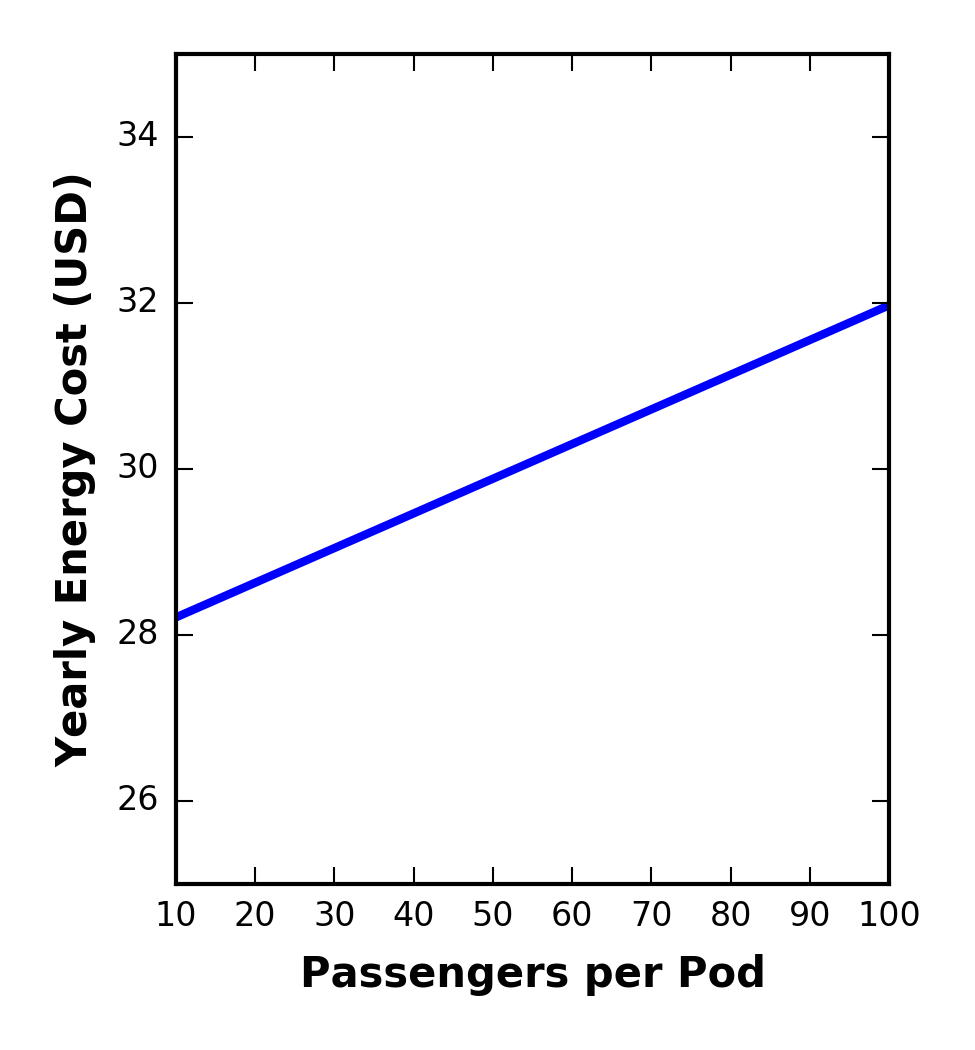
\includegraphics{../../images/graphs/capacity_trades/passengers_vs_energy.png}
	\caption{Yearly Energy Cost vs. Passengers per Pod}
	\label{fig:energy_cost_vs_passengers}
\end{figure}
\Cref{fig:energy_cost_vs_passengers} shows the relationship between yearly
energy consumption and the number of passengers per pod produced by the system model.
It is shown that, for the given operating condition, an order of magnitude
increase in pod capacity only results in a 15\% increase in yearly energy consumption.
This, in conjunction with the previously discussed structural analysis,
indicates that the cost associated with changing pod capacity is small.
This relationship is significant because it means that the Hyperloop operator
can specifically set the pod capacity to whatever value is necessary to meet a
particular market demand without costly changes in performance or design.
Furthermore, this makes it possible for future researchers to consider making
Hyperloop pods modular. It is possible that, instead of having one large pod
carrying a fixed number of passengers, the operator could have multiple pods
that carry a small number of passengers each link together until the capacity
of each individual flight reaches the value required by the market.
This would allow the Hyperloop to handle high densities of passengers during
peak travel times without having to increase pod frequency to prohibitive levels.
Then, during lighter travel times, the operator could link fewer pods together
to reduce the gross weight of each flight in order to reduce unnecessary energy consumption.
The performance of the Hyperloop system scales favorably with pod capacity,
which could potentially allow the system to be optimized to meet the demands
of the market with little cost to operator.
